%************************************************
\section{Conclusions and Future Work}\label{ch:conclusions}
%************************************************

To finish this document, we sum up some conclusions from the work done, and results 
obtained. We will also enumerate some future lines of research.

\subsection{Conclusions}


In the memory of this project we try to show the work done from the beginning, but we only showed our right decisions, and the information that is significant for the final result. The truth is that, aside from the information included in this paper, we have worked with other systems that ended up discarded. This isn't a negative aspect, because if we didn't, for example, study the Contiki OS, Cooja simulator and the compatible hardware, we could not be sure the development of a PoC for that system would be almost impossible in the time given.


With regard to the work presented, the flexibility of the computation offloading technique, identifying the key operations that can be delegated, and those ones that can't, has allowed us to define a general solution for the vast world of the Internet of Things. The IoT devices can operate as individual actors in the P2ABCE ecosystem, and when in need of performing computation offloading, the delegation server can also be a device considered into the IoT class.


% Resultados son válidos: feseability, problema de tiempo en sistemas de tiempo real
% Se han conseguido objetivos planteados
% Experiencia: qué era más tedioso, dificultades durante diseño y desarrollo
% Primera aproximación de este tipo ~~: más bien somos el future work de...
% Aplicación de procedimientos aprendidos/aplicados durante el TFG/carrera
% ^ Novelty


During the development, we had to investigate a lot of concepts related to IoT, smart cards, and even the insides of P2ABCE's code, to fix many existing bugs in the original project and minimize the amount of changes it had to undergo, in order to work with the IoT devices.% In the implementation chapter we give guidelines to port MULTOS applications, considering the particularities we encountered, that's why we can't consider it an \textit{instruction manual to port MULTOS apps}, but an interesting reading on how to confront a similar project. For example, if we wanted the Idemix implementation from \cite{vullers2013efficient}, previous to P2ABCE, in a IoT device, we could apply almost the same steps, obtaining a core functionality of Idemix for constrained devices in C.

Our PoC implementation demonstrates that this project is actually feasible, not by performing a simulation of an IoT device, like in \cite{vanet}. However, the use of third party libraries and no hardware acceleration support, makes the PoC too slow for certain cases, like real-time systems.

%Recalling the objectives listed in \autoref{objectives:section}, we think we accomplish them, except the implementation of a PoC in the most constrained device possible, where we used LEDE to ease our development, and the last objective, where we could have given a use to the PoC, and we leave as part of the future work. In spite of this negative auto-critic, we have to acknowledge that this is the first privacy-preserving ABC implementation for IoT, designed for extensibility, interoperability and maintenance.

%Finally, we are very thankful to IBM's grant for the \textit{Privacy Preserving Identity Management applied to IoT} project, which allowed us to get this far. 


\subsection{Future work}


%Due to the nature of the project, there exist many options to continue researching in this area.

On the design aspect, we mentioned a P2ABCE API to abstract the delegation process to other processes running in the IoT devices. To develop this API we should compare every possible solution proposed to decide on how to delegate to the server, e.g. REST, CoAP, RPC, and consider the security issues mentioned in previous sections, then we can define the API and implement it.

Also, now that an IoT device can perform P2ABCE operations, we could integrate it in a bigger project, like inside an IdM\footnote{Identity Management - KeyRock \url{https://catalogue.fiware.org/enablers/identity-management-keyrock}} system of FIWARE\footnote{\url{https://www.fiware.org/}}, to issue Idemix credentials to both users and IoT devices.% And once the identification is achieved in a privacy-preserving fashion, more applications should be researched, like how the IoT device could benefit from the ZKP cryptography to prove information not issued in its credential, by expanding the P2ABCE presentation policies.


On the implementation side, we would continue with a second PoC which aimed for more constrained devices, like Arduino systems. Another line of development could be to implement more P2ABCE functionality inside the IoT device, in order to delegate less on the P2ABCE server. It also would be interesting to compare the execution of the current PoC to a version with cryptographic hardware acceleration, for example, using Atmel's chips for SHA, AES and secure memory.



\begin{figure}[bth]
	\begin{center}
		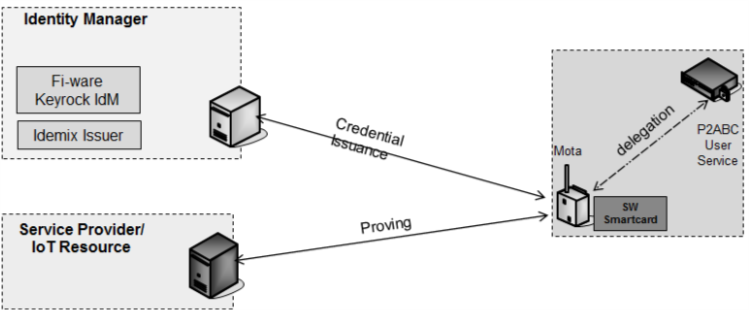
\includegraphics[width=0.8\linewidth]{gfx/fiware}
		\caption{IoT+Idemix Fi-Ware integration.}
	\end{center}
	\label{fig:fiware}
\end{figure}